\subsection{Rule 1: Convert Reentry Circuits to Activation Nodes}
Within the conduction network of the heart, there can be multiple pathways between two locations, forming conduction loops. If the timing parameters of the tissue along the loop satisfy certain property, there can be scenarios in which an depolarization wave circling the circuit. The circuits are referred to as \emph{Reentry Circuits}. Since the time interval for an activation wave to circle a reentry circuit is usually less than the intrinsic heart cycle length, the heart rate will be "`hijacked"' by the reentry circuit once the cycling is triggered, causing tachycardia. Reentry is the most common mechanism for tachycardia which can be modeled by our heart models \cite{vhm_embc10}. 

The effect of reentry tachycardia is that activation signals coming out of the circuit with cycle length equals to the sum of conduction delays of the conduction paths forming the circuit. It is therefore reasonable to model a reentry circuit as a self-activation node with the self-activation range equal to the sum of conduction delays. For more complex structures with multiple circuits, the self-activation range will be the minimum of the shortest circuit to the maximum of the longest circuit. The detailed rule description and implementation can be found in %\cite{regar_tech}.
%\begin{figure}[!h]
%\centering
%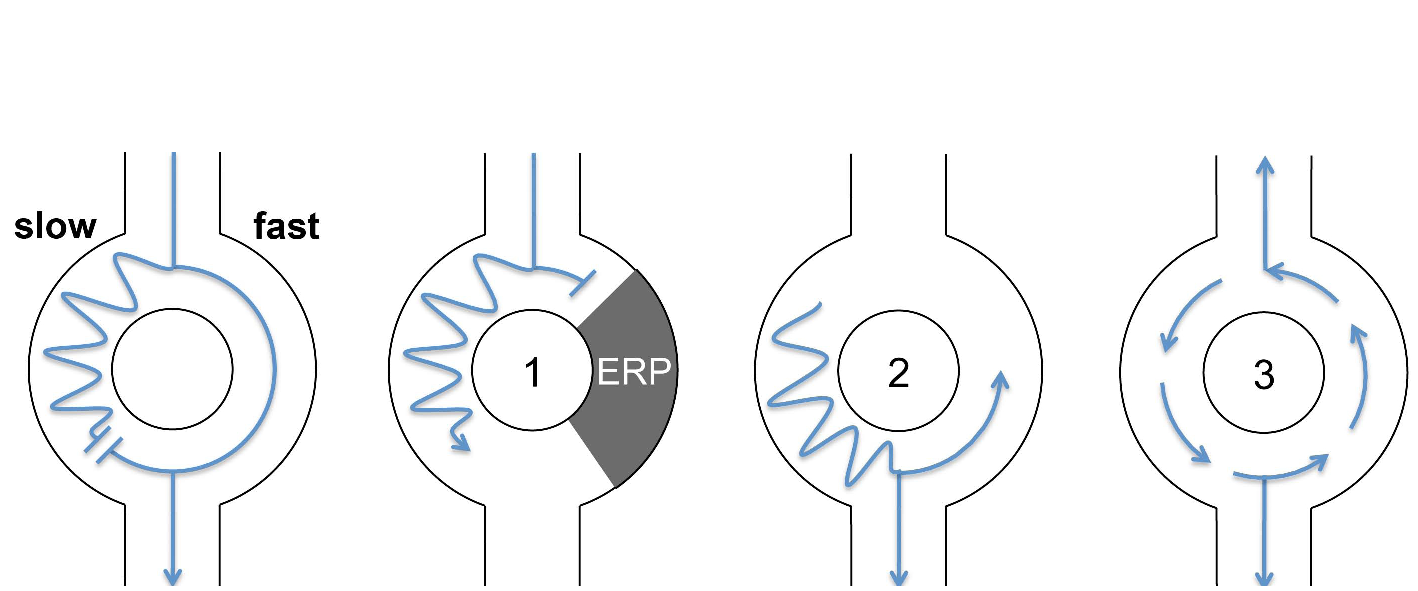
\includegraphics[width=0.6\textwidth]{figs/reentry.pdf}
%%\vspace{-5pt}
%\caption{\small Reentry Circuit}
%%\vspace{-15pt}
%\label{fig:reentry}
%\end{figure}
